\documentclass[a4paper]{article}
\usepackage{graphicx, hyperref, xcolor, gensymb, amssymb, mathtools, wrapfig, mathtools, microtype, lastpage, caption, titlesec, paracol, longtable, booktabs, cancel}
\usepackage[T2A, T1]{fontenc}
\usepackage[utf8]{inputenc}
\usepackage[russian, ukrainian]{babel}
\hypersetup{
    colorlinks,
    linkcolor={blue!20!black},
    citecolor={blue!50!black},
    urlcolor={blue!80!black}
}

\usepackage[left = 25mm, right = 10mm, top=20mm, bottom=20mm, bindingoffset=0cm]{geometry}

% КОМАНДИ

\newcommand{\fnt}{
\fontshape{n}
\fontsize{14pt} {19pt}
\linespread{0.8}
\selectfont
} % нормативний шрифт
\newcommand{\capfnt}{
    \fnt
} % норматичний шрифт для підписів (тимчасово співпадає зі звичайним шрифтом)

\newcommand{\tb}{
    \hspace*{10mm}
} % відступ у 5 символів "x" відповідно до ДСТУ
\newcommand{\tbln}{
    \newline 
    \tb
} % те ж саме, але з переносом рядка
\newcommand{\tbsp}{
    \vspace*{1ex}
    \tbln
} % те ж саме, але з додатковим відступом між рядками

% бібліографія
\usepackage[square,sort,comma,numbers]{natbib}
\renewcommand{\bibsection}{}
\usepackage{totcount}
\newtotcounter{citnum} 
% лічильник цитувань
\def\oldbibitem{} \let\oldbibitem=\bibitem
\def\bibitem{\stepcounter{citnum}\oldbibitem}

% лічильник зображень
\newtotcounter{graphnum}
\def\oldincludegraphics{} \let\oldincludegraphics=\includegraphics
\def\includegraphics{\stepcounter{graphnum}\oldincludegraphics}

% лічильник таблиць (НЕАВТОМАТИЧНИЙ!!!)
\newtotcounter{tabnum}

% лічильник додатків (НЕАВТОМАТИЧНИЙ!!!)
\newtotcounter{dodnum}

% нумерація сторінок
\usepackage{fancyhdr}
\pagestyle{fancy}
\fancyhf{}
\renewcommand{\headrulewidth}{0pt}
\setlength{\headheight}{15.3pt}
\fancyhead[R]{\fnt \thepage}

% виноски
\renewcommand{\thefootnote}{\large\arabic{footnote})~}
\renewcommand{\footnoterule}{\rule{20mm}{0.4pt} \vspace*{0.5ex}}
% \newcommand{\vyn}[2]{
%     \footnote[#1]{\large #2}
% } % створити виноску

\let\oldFootnote\footnote
\renewcommand{\footnote}[1]{
    \oldFootnote{\large #1}
} % перегрузка виноски

\providecommand{\tightlist}{%
  \setlength{\itemsep}{0pt}\setlength{\parskip}{0pt}}

% підписи малюнків/таблиць
\captionsetup[figure]{name={\fnt Рисунок~},labelsep=period}
\captionsetup[table]{name={\fnt Таблиця~},labelsep=period}

% markdown strikeouts
\usepackage{soul}

% codeblocks
\usepackage{minted}

% enumeration
\usepackage[shortlabels]{enumitem}

\titleformat*{\section}{\fnt\LARGE\bfseries}
\titleformat*{\subsection}{\fnt\Large\bfseries}
\titleformat*{\subsubsection}{\fnt\Large}

\begin{document}
\thispagestyle{empty} % [A]:for cropping
% ------------
% source: https://tex.stackexchange.com/questions/173651/need-help-to-create-such-a-beautiful-title-page
\begingroup
\centering
\obeylines
\topskip 0pt % source: https://tex.stackexchange.com/questions/2326/vertically-center-text-on-a-page
\vspace*{\fill}
\textbf{
\LARGE 
\LARGE 
\vspace{100pt}
\LARGE 
\Large 
\Large 
\Large 
\huge 
\vspace{50pt}
\large 
\large 
\large 
\large 
\vspace*{\fill}
\hspace{\fill}\large  \rule{20mm}{0.4pt}
\vspace{10pt}
}
\endgroup
% ------------
\newpage
\tableofcontents

\newpage
\fnt
Here's a quick rundown of supported markdown syntax:
\section{Headers}

\textbf{Up to 6 deep}

\tb Inline math: $y = x^2\qquad \text{- is a parabola equation}$
\tbln Display math:
\begin{equation}
\Gamma(z) = \int\limits_{0}^{+\infty} \exp(-t) t^{z-1} dt \qquad \text{- це Euler's Gamma-function definition}
\label{eq:gamma_function}
\end{equation}

\tb Page breaks:
\clearpage

\tb This text must appear on the next page
\tbln Figures (take note of the caption and ident):
\begin{figure}[h!]
\centering
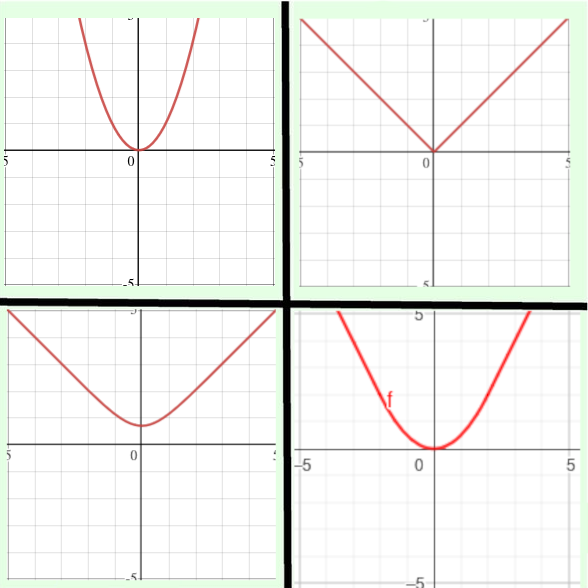
\includegraphics[width=0.4\textwidth]{examples/basic_syntax/images/loss_meme.png}
\caption{\capfnt These are all loss functions, technically making this image a loss meme}
\label{fig:loss_meme}
\end{figure}

\tb Tables:
\begin{table}[h!]
\fnt
\begin{center}
\begin{tabular}{|c|c|}\hline
 Number of appendages &  Name\\ \hline
\hline
 1 &  Monopedal\\ \hline
 2 &  Bipedal\\ \hline
 3 &  Tripedal\\ \hline
 4 &  Quadropedal\\ \hline
 5 &  Pentapedal\\ \hline
 6 &  Hexapedal\\ \hline
 7 &  Heptopedal\\ \hline
 8 &  Octopedal\\ \hline
 9 &  why.\\ \hline
 1001 &  are you sure\\ \hline
 $\omega_0$ &  are you ok?\\ \hline
 $\zeta_1$ &  cracker\\ \hline
\end{tabular}
\stepcounter{tabnum}
\caption{\capfnt Source: trust \textbf{me}}
\label{tab:pedals}
\end{center}
\end{table}

\tb Hyper references: \href{https://www.somewebsite.com/}{some website}
\tbln Footnotes: say, I need to explain this text, but not include the actual explanation right where I write it\footnotemark[1]\footnotetext[1]{You can absolutely do this! \textit{Note}, that despite this footnote definition is on a separate page at the end, actual document output includes the footnote in a more convenient spot.}
\tbln Object references: this refers to table: \ref{tab:pedals}, this refers to figure: \ref{fig:loss_meme}, an this one to the equation at the beginning: \ref{eq:gamma_function}.
\tbln Lists are supported too; Here's a bullet list:
\begin{itemize}
\item First item
\item Second item
\item Third item
\end{itemize}
\tb Here's an enumeration:
\begin{enumerate}
\item First item
\item Second item
\item Third item
\end{enumerate}
\tb Here are alphabetic enumerations (latin and cyrillic are only supported, for now)
\begin{enumerate}
\item[a.] First item
\item[b.] Second item
\item[c.] Third item
\end{enumerate}
\begin{enumerate}
\item[а.] First item
\item[б.] Second item
\item[в.] Third item
\end{enumerate}
\tb Cyrillic implementation detail: наразі у якості порядку елементів береться буквально 'а'..'я'. Тобто, згідно з \href{https://en.wikipedia.org/wiki/Cyrillic_(Unicode_block)}{таблицею юнікоду}, тут поки що реалізовано терористичний алфавіт:
\begin{enumerate}
\item[а.] Перший елемент
\item[б.] Другий елемент
\item[в.] Третій елемент
\item[г.] Четвертий елемент
\item[д.] Шостий елемент (не вистачає ґ)
\end{enumerate}
\tb Це може змінитись у майбутньому, тож краще поки що утриматись від використання кириличних списків.
\tbln Finally, code blocks are supported:
\begin{minted}[linenos, mathescape, autogobble, breaklines]{lua}
print("Hello lua!")
function fact (n)
    if n == 0 or n == 1 then
        return 1
    else
        return n * fact(n-1)
    end
end

print(fact(7))
\end{minted}


\begin{minted}[linenos, mathescape, autogobble, breaklines]{rust}
#[repr(transparent)]
#[derive(Debug, derive_more::From, derive_more::Deref, derive_more::DerefMut)]
pub struct Equivalent<T>(pub T);

impl<T> PartialEq for Equivalent<T> {
    fn eq(&self, _: &Self) -> bool {
        true
    }
}

impl<T> Eq for Equivalent<T> {}

// This is a real type used in this project's codebase to allow error comparison for testing
// Although I might decide to remove it in the future
\end{minted}


\tb These blocks are powered by \href{https://github.com/gpoore/minted}{minted}, so to get full list of supported languages, check their docs out.
\tbln This is all of the markdown syntax supported for now. However, there's an \textit{otherside} to `kyomato`'s capabilities - namely, `ayano` blocks.
\clearpage


\end{document}